\chapter{Desarrollo de APIs}

En este capítulo se hablará sobre las diferentes librerías (APIs) que se han realizado en este proyecto, explicando detalladamente la estructura de cada una de ellas.

Por último, se hará especial énfasis en el plugin de Net2Plan desarrollado, en el cual se han integrado las difrentes APIs mencionadas anteriormente.


\section{J-OSM Client}
\label{sec:osmclient}

\section{ONOS Client}
\label{sec:onosclient}

\section{OpenStack Client}
\label{sec:openstackclient}

\section{Net2Plan: NFV Management Plugin}
\label{sec:nfvplugin}

\begin{figure}[!ht]
	\centering
	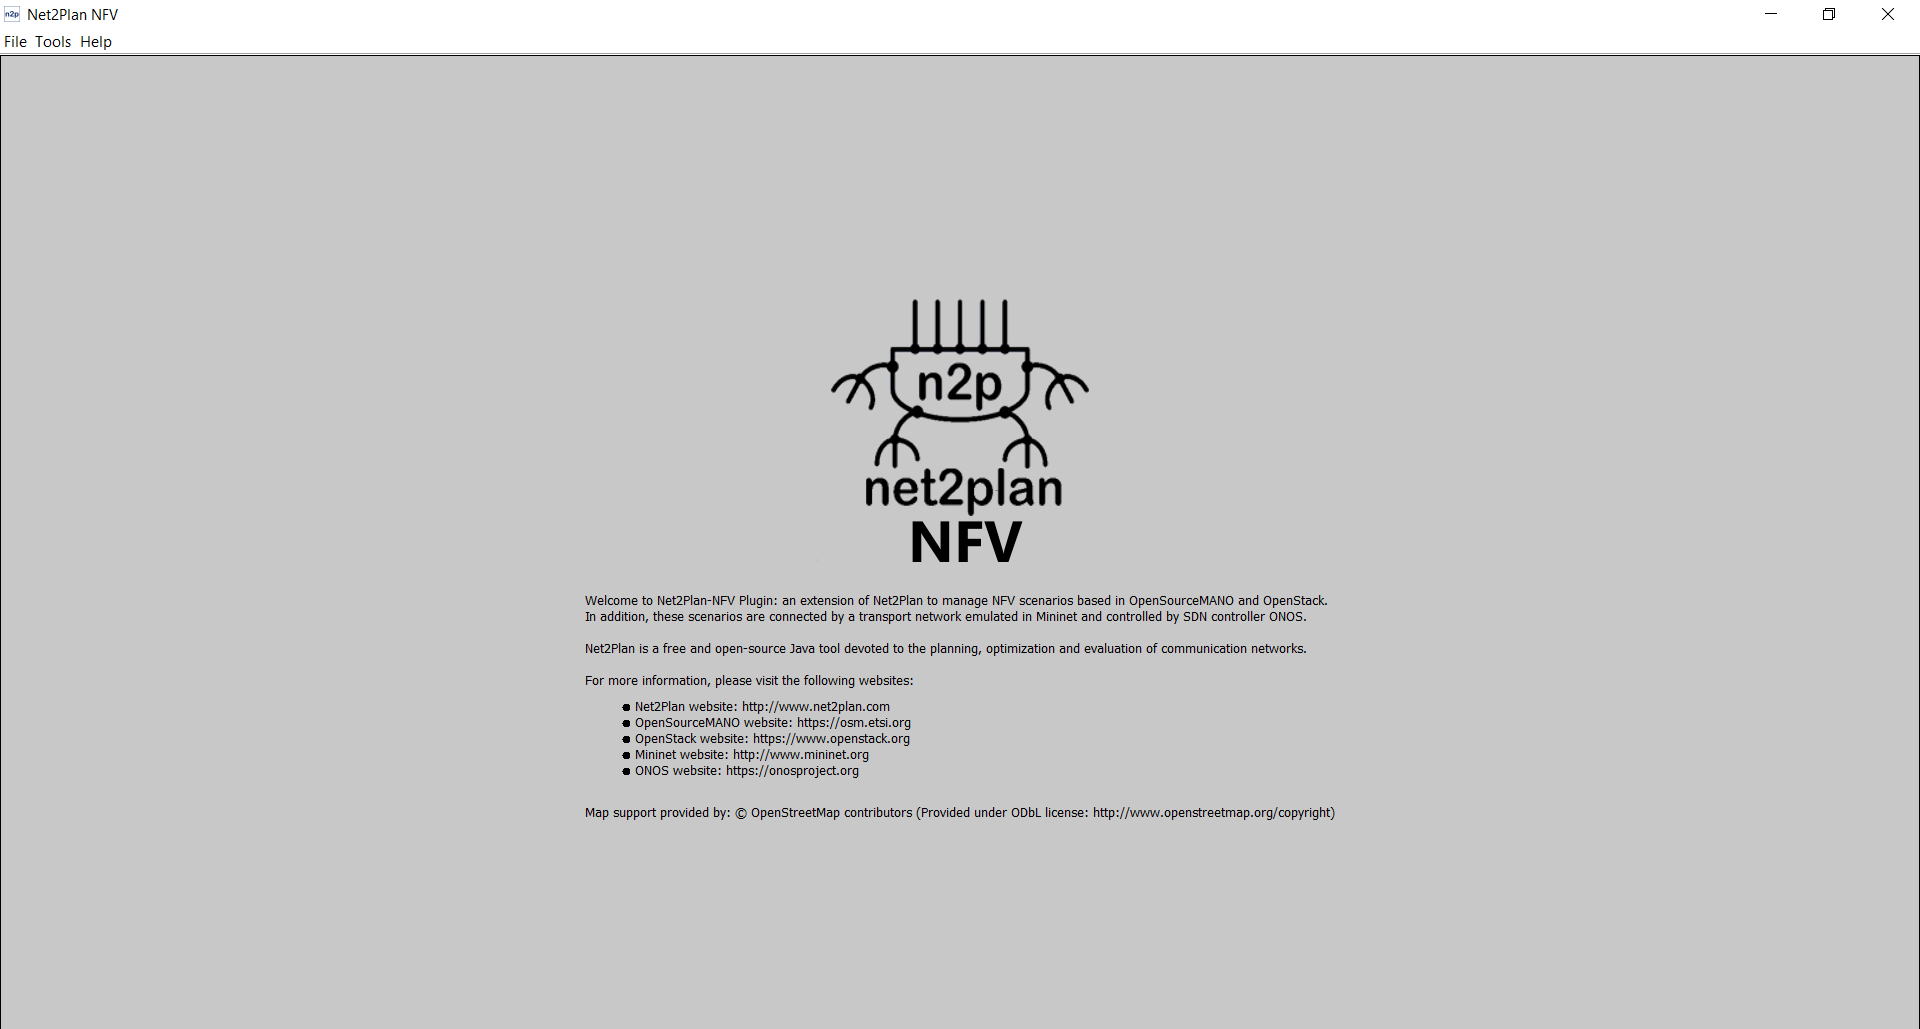
\includegraphics[width=0.8\linewidth]{imagenes/nfvpluginmain}
	\caption{Página de inicio de la extensión Net2Plan-NFV}
	\label{fig:nfvpluginmain}
\end{figure}

\begin{figure}[!ht]
	\centering
	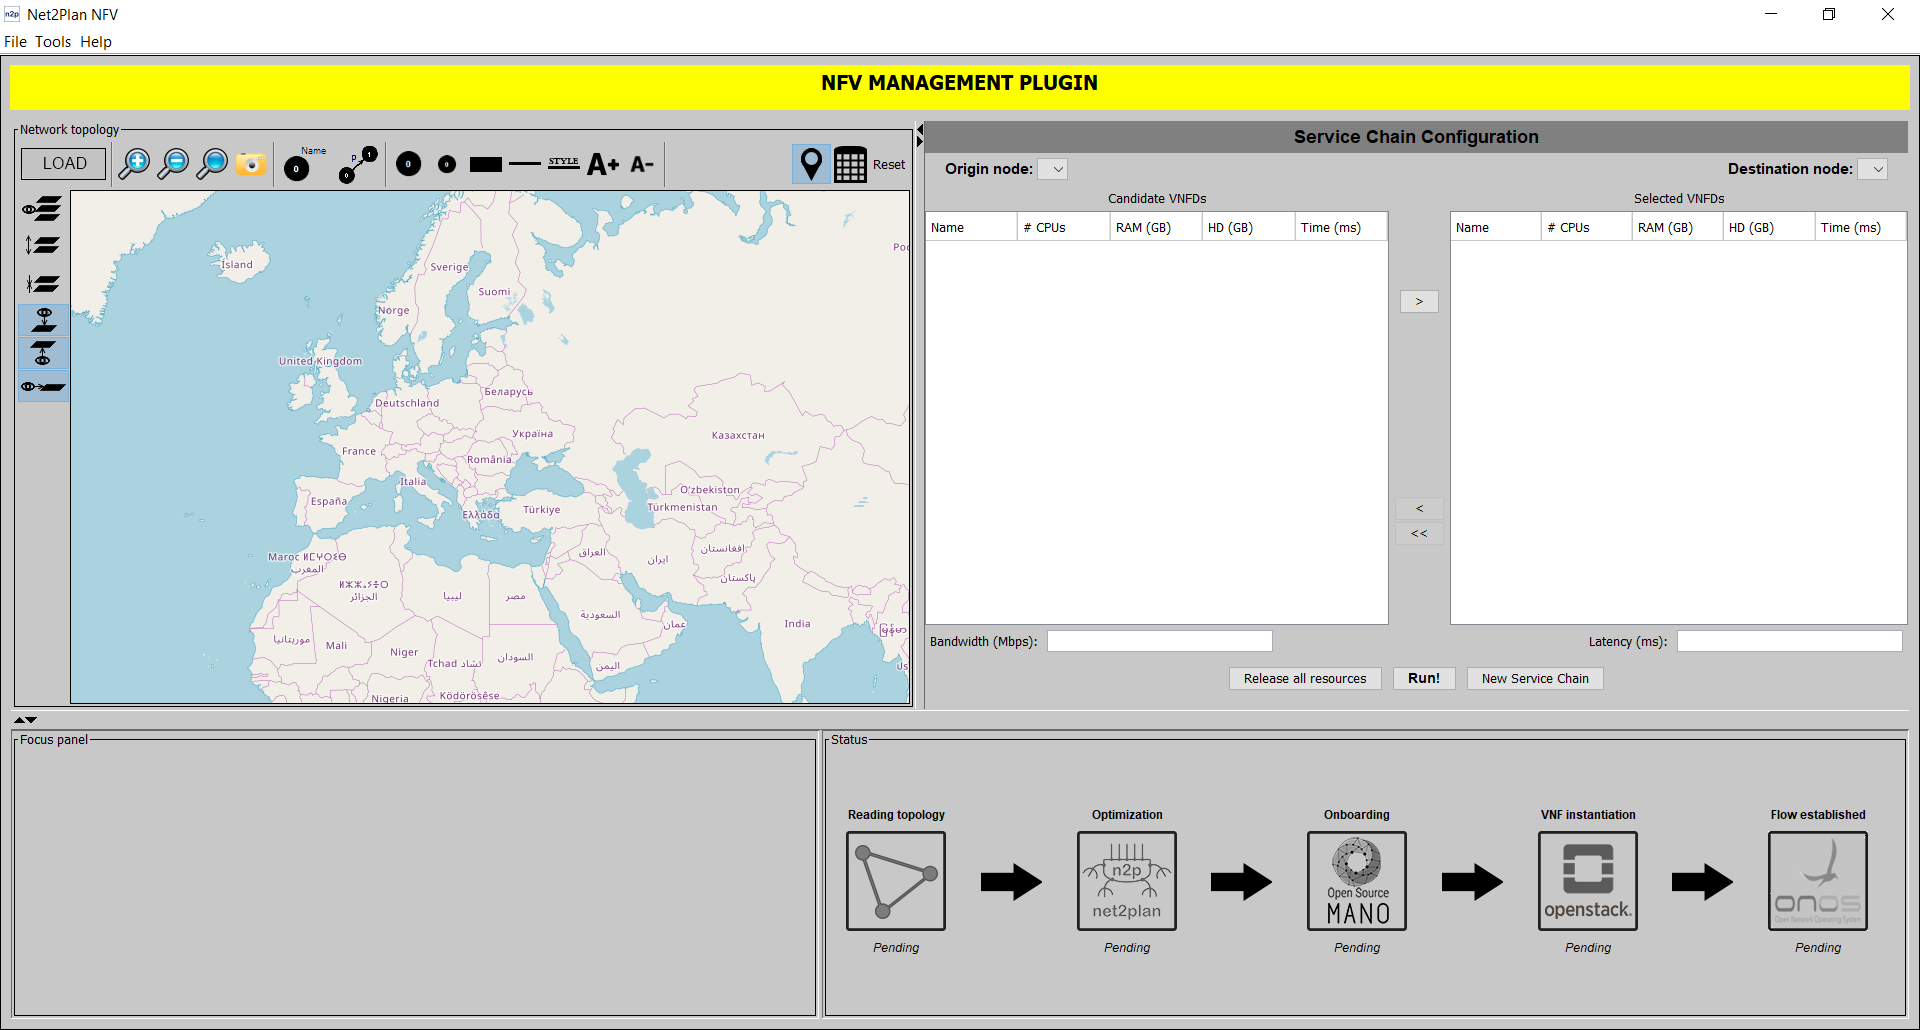
\includegraphics[width=0.8\linewidth]{imagenes/nfvplugin_dashboard}
	\caption{Página de inicio del Plugin NFV-Management}
	\label{fig:nfvplugindash}
\end{figure}


En la figura \ref{fig:nfvpluginmain} se puede observar la vista que ofrece el plugin de Net2Plan desarrollado para la prueba de concepto.



\cleardoublepage